\documentclass[12pt,a4paper]{article}
% Fix for fancyhdr headheight error
\setlength{\headheight}{14.5pt}
% --- PACKAGES ---
% --- ENCODING & FONTS ---
\usepackage[utf8]{inputenc}
\usepackage[T1]{fontenc}
\usepackage{lmodern}          % Modern font (alternative to Times)
% \usepackage{times}          % OPTIONAL: Classic serif font (comment if using lmodern)

\usepackage{pgf-pie}
\usepackage{pgfplots}
\usepackage{subcaption}
\usepackage{xcolor}
\usepackage{colortbl}
\usepackage{multirow}
\usepackage{booktabs}
\usepackage{siunitx}
\usepackage{float}

% --- PAGE LAYOUT ---
\usepackage[a4paper, left=0.75in, right=0.75in, top=1in, bottom=1in]{geometry}
\usepackage{parskip}          % Paragraphs with spacing instead of indentation
\usepackage{setspace}         % For line spacing

% --- MATHEMATICS ---
\usepackage{amsmath, amsfonts, amssymb}

% --- GRAPHICS & FIGURES ---
\usepackage{graphicx}
\usepackage{caption}
\usepackage{float}
\usepackage{array, longtable, colortbl}
\usepackage{tabularx}

% --- COLORS ---
\usepackage[table]{xcolor}
\usepackage{xcolor}           % General color usage

% --- TIKZ & DIAGRAMS ---
\usepackage{tikz}
\usetikzlibrary{
  shapes.geometric,
  arrows.meta,
  positioning,
  fit,
  backgrounds,
  shapes.multipart
}

% --- PLOTS & CHARTS ---
\usepackage{pgf-pie}          % Pie charts
\usepackage{pgfplots}         % Graphs and plots
% Set pgfplots compatibility for modern features
\pgfplotsset{compat=1.18}

% --- DOCUMENT STRUCTURE ---
\usepackage{titlesec}         % Custom section titles
\usepackage{tocloft}          % Table of contents formatting
\usepackage{enumitem}         % Better lists

% --- HEADER, FOOTER & LINKS ---
\usepackage{fancyhdr}         % Custom headers/footers

% --- BIBLIOGRAPHY ---
\usepackage[numbers,sort&compress]{natbib}  % For references with numerical citations
\bibliographystyle{plainnat}  % Compatible style with natbib
\usepackage[many]{tcolorbox}
\tcbuselibrary{skins,breakable}

% --- Code listings for source code in Appendix ---
\usepackage{listings}
\lstset{
    language=Python,
    basicstyle=\ttfamily\small,
    breaklines=true,
    showstringspaces=false,
    numbers=left,
    numberstyle=\tiny\color{gray},
    frame=single,
    captionpos=b,
    keywordstyle=\color{blue},
    commentstyle=\color{green!60!black},
    stringstyle=\color{purple},
    rulecolor=\color{black!20},
    backgroundcolor=\color{black!5}
}

% --- Load hyperref last ---
\usepackage{hyperref}         % Clickable links


% --- COLORS ---
\definecolor{RoyalBlue}{RGB}{0, 70, 140}
\definecolor{RUETRed}{RGB}{179, 0, 0}
\definecolor{LightGray}{RGB}{248, 249, 250}
\definecolor{DarkGray}{RGB}{52, 58, 64}
\definecolor{AccentBlue}{RGB}{13, 110, 253}
\definecolor{ModernGray}{RGB}{108, 117, 125}
\definecolor{lightgreen}{RGB}{200, 255, 200}
\definecolor{lightred}{RGB}{255, 200, 200}

% Define modern color palette
\definecolor{primary}{RGB}{41, 128, 185}
\definecolor{secondary}{RGB}{52, 152, 219}
\definecolor{accent}{RGB}{231, 76, 60}
\definecolor{success}{RGB}{46, 204, 113}
\definecolor{warning}{RGB}{241, 196, 15}
\definecolor{darkgray}{RGB}{52, 73, 94}
\definecolor{lightgray}{RGB}{236, 240, 241}
\definecolor{purple}{RGB}{155, 89, 182}
\definecolor{orange}{RGB}{230, 126, 34}
\definecolor{teal}{RGB}{26, 188, 156}
\definecolor{OliveGreen}{RGB}{85, 107, 47}

\definecolor{outputbg}{RGB}{45, 45, 45} % Dark background for output

% --> ADDED for the blue info box
% --> Define colors for code boxes and result boxes
\definecolor{reportgreen}{RGB}{230, 245, 230}
\definecolor{reportdarkgreen}{RGB}{50, 120, 50}
\definecolor{outputbg}{RGB}{45, 45, 45} % Dark background for output
\definecolor{infoboxbg}{RGB}{235, 245, 255}
\definecolor{infoboxborder}{RGB}{70, 130, 180}
% --> ADDED: Define the blue info box style
\newtcolorbox{infobox}{
  colback=infoboxbg,
  colframe=infoboxborder,
  boxrule=0.5pt, % thin border for sides/bottom
  borderline north={1.5pt}{0pt}{infoboxborder}, % thicker top border
  arc=0mm,       % sharp corners
  left=5mm, % Add some padding
  top=3mm,
  bottom=3mm
}

% --> Define style for code listings (like Listing 2, 3 in friend's report)
\lstdefinestyle{code}{
    basicstyle=\ttfamily\small,
    numbers=left,
    numberstyle=\tiny\color{gray},
    numbersep=5pt,
    frame=none,
    breaklines=true,
    keywordstyle=\color{blue},
    commentstyle=\color{OliveGreen},
    stringstyle=\color{purple},
    showstringspaces=false
}
\lstset{style=code} % Set default listing style

% --> Define the green result box
\newtcolorbox{resultbox}[2][]{
    enhanced,
    attach boxed title to top center={yshift=-2mm},
    colback=reportgreen,
    colframe=reportdarkgreen,
    colbacktitle=reportgreen,
    coltitle=black,
    boxed title style={size=small,colframe=reportdarkgreen},
    title={#2},
    fonttitle=\bfseries
}

% --- FONT & STYLING ---
\renewcommand{\familydefault}{\sfdefault}  % Use sans-serif font
\titleformat{\section}{\fontsize{20}{24}\selectfont\bfseries\color{RoyalBlue}}{\thesection}{1em}{}
\titleformat{\subsection}{\fontsize{16}{20}\selectfont\bfseries\color{RoyalBlue}}{\thesubsection}{1em}{}
\titleformat{\subsubsection}{\fontsize{13}{16}\selectfont\bfseries\color{RoyalBlue}}{\thesubsubsection}{1em}{}

% TOC Styling
\renewcommand{\cfttoctitlefont}{\color{black}\Huge\bfseries}
\renewcommand{\cftsecfont}{\color{RoyalBlue}}
\renewcommand{\cftsecpagefont}{\color{RoyalBlue}}
\renewcommand{\cftsubsecfont}{\color{RoyalBlue}}
\renewcommand{\cftsubsecpagefont}{\color{RoyalBlue}}

% Header and Footer
\pagestyle{fancy}
\fancyhf{}
\fancyhead[C]{\textit{Data Mining Report}}
\fancyfoot[C]{\thepage}
\renewcommand{\headrulewidth}{0.4pt}
\renewcommand{\footrulewidth}{0pt}

% Hyperlink Styling
\hypersetup{
    colorlinks=true,
    linkcolor=RoyalBlue,
    filecolor=magenta,
    urlcolor=cyan,
    pdftitle={Data Mining Report},
    pdfpagemode=FullScreen,
    pdfborder={0 0 0},
}

% --- Define a global style for all plots for consistency ---
\pgfplotsset{
    every axis/.append style={
        axis x line=bottom,
        axis y line=left,
        label style={font=\bfseries},
        title style={font=\large\bfseries, yshift=1em},
        tick label style={font=\small},
        legend style={font=\small, at={(0.5,-0.2)}, anchor=north, legend columns=-1},
    }
}

% Modern title page with geometric design
\newcommand{\maketitlepage}{
    \begin{titlepage}
        \begin{tikzpicture}[remember picture,overlay]
            \fill[RoyalBlue!10] (current page.north west) rectangle ([yshift=-2.2cm]current page.north east);
            \fill[AccentBlue!5] ([yshift=-14cm]current page.north west) rectangle ([yshift=-16.2cm]current page.north east);
            \fill[RoyalBlue!15] ([xshift=2cm,yshift=-2cm]current page.north west) circle (1.2cm);
            \fill[AccentBlue!15] ([xshift=-2cm,yshift=-15.2cm]current page.north east) circle (0.9cm);
        \end{tikzpicture}

        \centering
        \vspace*{0.6cm}

        % Logo (only include if file exists)
        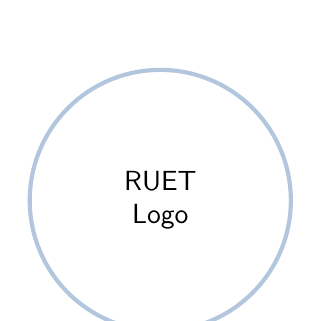
\begin{tikzpicture}
            \node[circle, draw=RoyalBlue!30, line width=1.5pt, inner sep=6pt] at (0,0) {
                 \IfFileExists{RUET_logo.png}{\includegraphics[width=2.7cm]{RUET_logo.png}}{\begin{minipage}{2.7cm}\centering RUET \\ Logo \end{minipage}}
            };
        \end{tikzpicture}

        \vspace{0.6cm}
        {\fontsize{15.5}{17}\selectfont\bfseries\textcolor{RUETRed}{RAJSHAHI UNIVERSITY OF ENGINEERING \& TECHNOLOGY}\par}
        \vspace{0.2cm}
        {\fontsize{13.5}{16}\selectfont\textcolor{DarkGray}{Department of Computer Science and Engineering}\par}

        \vspace{1.5cm}
        % Title Block
        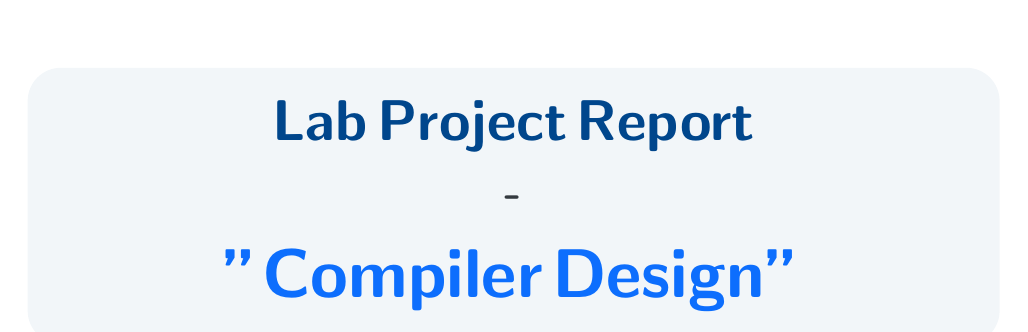
\begin{tikzpicture}
            \node[rectangle, fill=RoyalBlue!5, rounded corners=12pt, inner sep=12pt, text width=11.5cm, align=center] at (0,0) {
                {\fontsize{21}{24}\selectfont\bfseries\textcolor{RoyalBlue}{Lab Project Report}\par}
                \vspace{0.15cm}
                {\fontsize{16}{20}\selectfont\bfseries\textcolor{DarkGray}{-}\par}
                \vspace{0.15cm}
                {\fontsize{24}{28}\selectfont\bfseries\textcolor{AccentBlue}{"Compiler Design"}\par}
            };
        \end{tikzpicture}

        \vspace{1.8cm}
        % Submission info
        \begin{minipage}[t]{0.45\textwidth}
            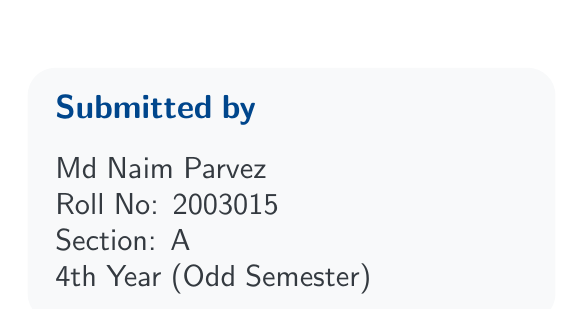
\begin{tikzpicture}
                \node[rectangle, fill=LightGray, rounded corners=10pt, inner sep=10pt, text width=6cm] at (0,0) {
                    {\fontsize{13}{15}\selectfont\bfseries\textcolor{RoyalBlue}{Submitted by}\par}
                    \vspace{0.3cm}
                    {\fontsize{11}{13}\selectfont\textcolor{DarkGray}{
                        Md Naim Parvez\\
                        Roll No: 2003015\\
                        Section: A\\
                        4th Year (Odd Semester)
                    }\par}
                };
            \end{tikzpicture}
        \end{minipage}
        \hfill
        \begin{minipage}[t]{0.50\textwidth}
            
\begin{tikzpicture}
                \node[rectangle, fill=AccentBlue!5, rounded corners=10pt, inner sep=10pt, text width=6cm] at (0,0) {
                    {\fontsize{13}{15}\selectfont\bfseries\textcolor{RoyalBlue}{Submitted to}\par}
                    \vspace{0.3cm}
                    {\fontsize{11}{13}\selectfont\textcolor{DarkGray}{
                        Farjana Parvin\\
                        Assistant Professor\\
                        Department of CSE\\
                        Rajshahi University of Engineering \& Technology\\
                        \vspace{0.3cm}
                    }\par}
                };
            \end{tikzpicture}
        \end{minipage}

        \vspace{1.2cm}
        % Course Info
        
\begin{tikzpicture}
            \node[rectangle, fill=RoyalBlue!10, rounded corners=10pt, inner sep=12pt, align=center, text width=13cm] at (0,0) {
                {\fontsize{13}{16}\selectfont\bfseries\textcolor{RoyalBlue}{Course Code: } \textcolor{DarkGray}{4102}}\\[0.2cm]
                {\fontsize{13}{16}\selectfont\bfseries\textcolor{RoyalBlue}{Course Title: } \textcolor{DarkGray}{Compiler Design Sessional}}
            };
        \end{tikzpicture}

        \vspace{0.8cm}
    \end{titlepage}
}


\begin{document}

% --- TITLE PAGE ---
\maketitlepage
\thispagestyle{empty} % No header/footer on the title page

\newpage
% --- TABLE OF CONTENTS ---
\pagenumbering{roman} % Roman numerals for ToC, Abstract etc.
\phantomsection % Helps hyperref create proper links
\tableofcontents

% --- LIST OF FIGURES ---
\newpage
\phantomsection % Helps hyperref create proper links
\pagenumbering{arabic} % Arabic numerals for main content
\setcounter{page}{1} % Start main content page numbering from 1
% ============= CHAPTER 1: INTRODUCTION =============
\section{Introduction}

\subsection*{Overview}
Compiler design is a fundamental area of computer science that bridges high-level programming languages and machine-level execution. This project implements a complete compiler for a custom programming language with Bengali-inspired keywords, demonstrating the entire compilation pipeline from source code to assembly language.


\subsection*{Objectives}
The primary objectives of this project are:
\begin{itemize}
    \item Design and implement a lexical analyzer using Flex
    \item Develop a parser using Bison for syntax analysis
    \item Create a symbol table for variable management
    \item Generate intermediate code representation
    \item Produce x86 assembly code output
\end{itemize}


% ============= CHAPTER 2: LITERATURE REVIEW =============
\section{Literature Review}

\subsection*{Compiler Structure}
A compiler typically consists of several phases working in sequence. The front-end phases include lexical analysis, syntax analysis, and semantic analysis, while the back-end phases handle intermediate code generation, optimization, and target code generation. This project implements the essential phases required for a functional compiler.

\subsection*{Lexical Analysis}
Lexical analysis is the first phase of compilation, where the source code is read as a stream of characters and grouped into meaningful sequences called tokens. Tools like Flex (Fast Lexical Analyzer) automate this process by using regular expressions to define token patterns.

\subsection*{Syntax Analysis}
Syntax analysis, or parsing, verifies that the token sequence conforms to the language's grammar rules. Parser generators like Bison use context-free grammars to build parse trees and detect syntax errors. The parser works in conjunction with the lexer to build a hierarchical representation of the program structure.

\subsection*{Code Generation}
Code generation translates the intermediate representation into target machine code. For this project, x86 assembly language serves as the target, requiring careful management of registers, memory, and the runtime stack.


% ============= CHAPTER 4: IMPLEMENTATION =============
\section{Implementation}

\subsection*{input.txt}

\begin{lstlisting}[caption={Input Test Program (Input.txt)}]
FUNC main ()
start
    mone_kori a <-- integer
    mone_kori b <-- integer
    a equal 12
    b equal 13 jog a
    print_kori b
end
\end{lstlisting}


% ============= CHAPTER 5: TESTING =============
\section{Output Analysis}


\subsection*{Lexical Analysis Output}
The lexer successfully tokenizes the input:

\begin{lstlisting}[caption={Lexical Analysis Output}]
Token: FUNC
Token: ID (main)
Token: (
Token: )
Token: start
Token: mone_kori
Token: ID (a)
Token: <--
Token: integer
Token: mone_kori
Token: ID (b)
Token: <--
Token: integer
Token: ID (a)
Token: equal
Token: ICONST (12)
Token: ID (b)
Token: equal
Token: ICONST (13)
Token: jog
Token: ID (a)
Token: print_kori
Token: ID (b)
Token: end
\end{lstlisting}
\begin{figure}[H]
    \centering
    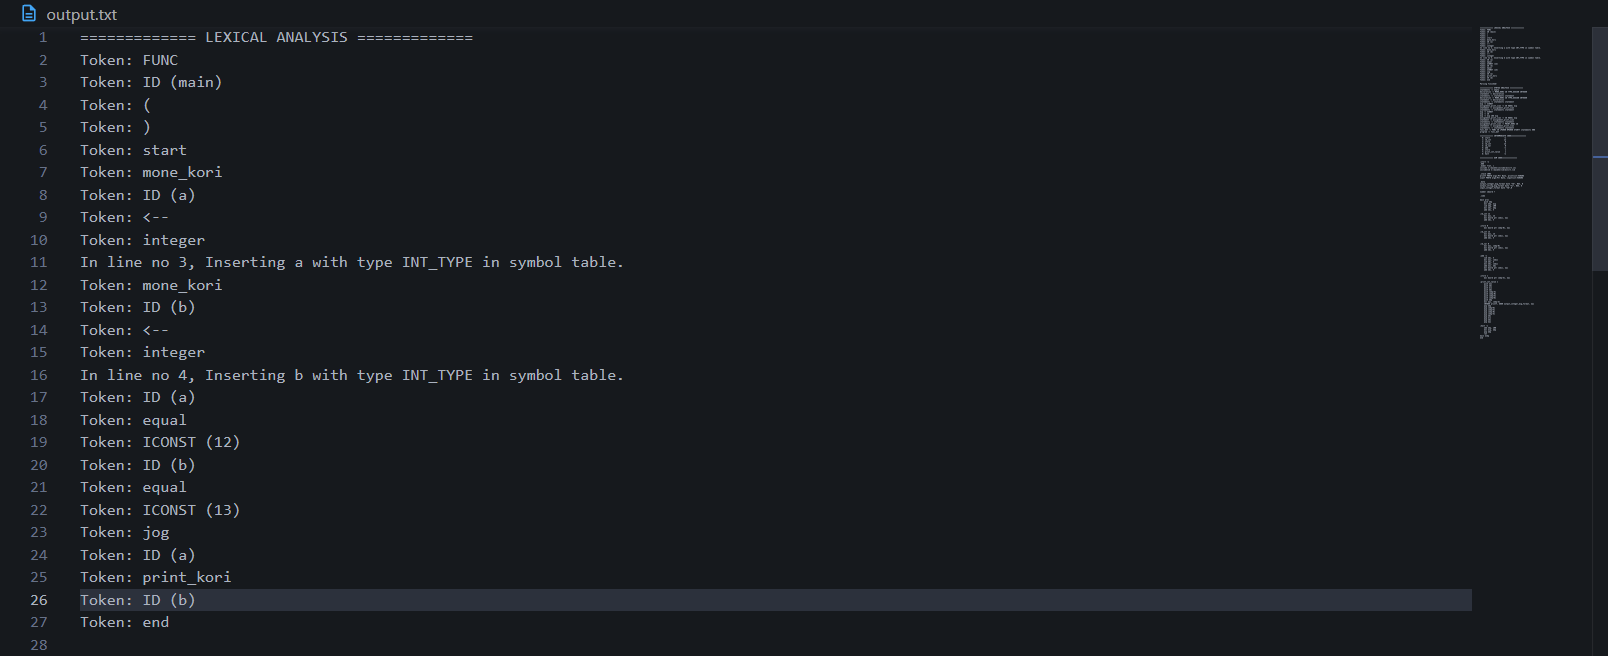
\includegraphics[width=0.9\textwidth]{token.png}
    \caption{Lexical Analysis Output}
    \label{fig:label}
\end{figure}
\subsection*{Syntax Analysis Output}
The parser generates the parse tree:

\begin{lstlisting}[caption={Parse Tree}]
statements -> empty
declaration -> MONE_KORI ID TYPE_ASSIGN INTEGER
statement -> declaration
statements -> statements statement
declaration -> MONE_KORI ID TYPE_ASSIGN INTEGER
statement -> declaration
statements -> statements statement
exp -> ICONST

assignment_print_scan -> ID EQUAL exp
statement -> assignment_print_scan
statements -> statements statement
exp -> ICONST
exp -> ID
exp -> exp JOG exp

assignment_print_scan -> ID EQUAL exp
statement -> assignment_print_scan
statements -> statements statement
assignment_print_scan -> PRINT_KORI ID
statement -> assignment_print_scan
statements -> statements statement
func_def -> FUNC ID LPAREN RPAREN STARTT statements END
program -> func_def
\end{lstlisting}
\begin{figure}[H]
    \centering
    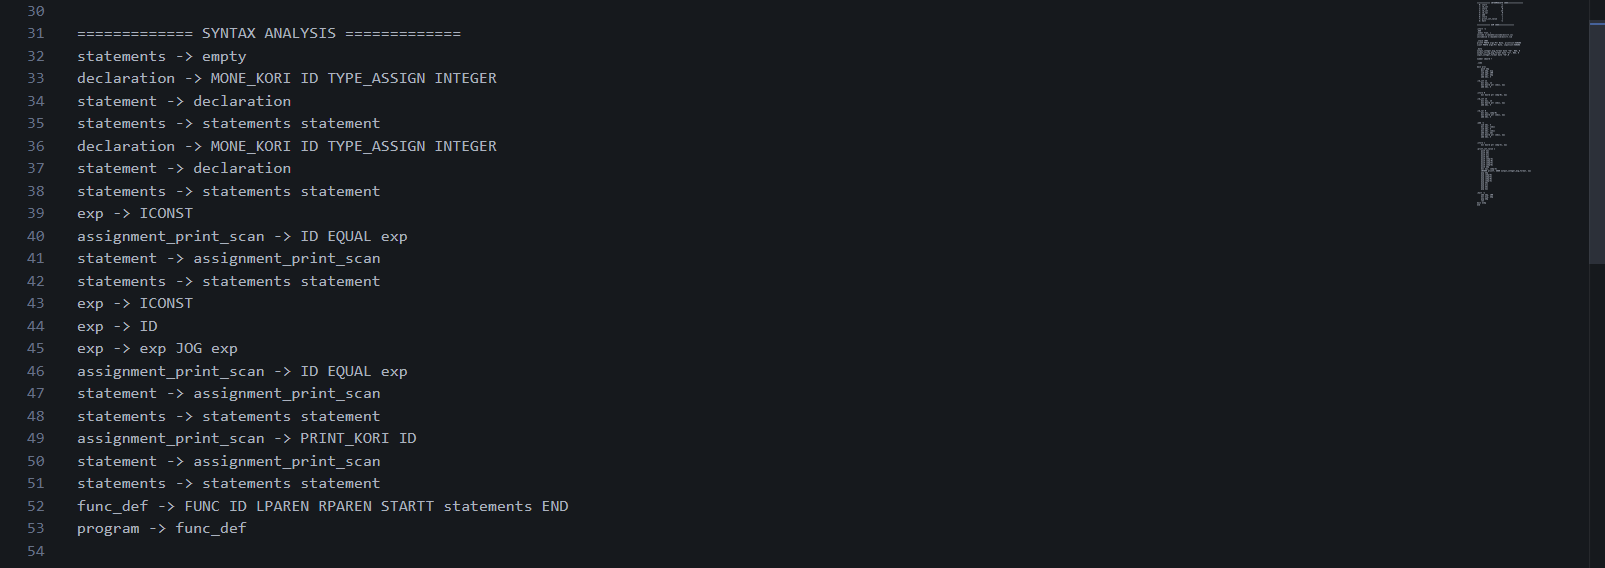
\includegraphics[width=0.9\textwidth]{parsetree.png}
    \caption{Syntax Analysis Output}
    \label{fig:label}
\end{figure}
\subsection*{Intermediate Code}
The generated intermediate code:

\begin{lstlisting}[caption={Intermediate Code}]
0: start -1
1: ld_int 12
2: store 0
3: ld_int 13
4: ld_var 0
5: add -1
6: store 1
7: print_int_value 1
8: halt -1
\end{lstlisting}
\begin{figure}[H]
    \centering
    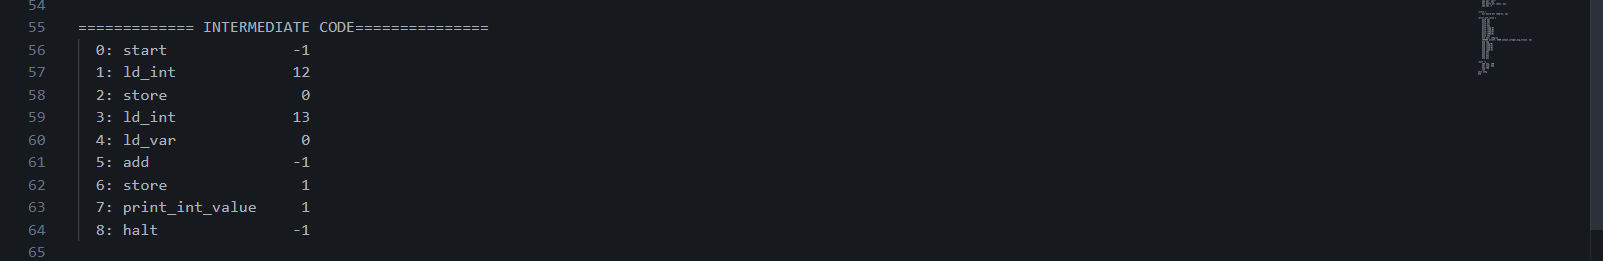
\includegraphics[width=0.9\textwidth]{IMcode.png}
    \caption{Intermediate Code}
    \label{fig:label}
\end{figure}
\subsection*{Assembly Code Output}
The final x86 assembly code (excerpt):

\begin{lstlisting}[language={[x86masm]Assembler}, caption={Generated Assembly Code}]
.686
.model flat, c
.stack 100h
.data
output_integer_msg_format byte "%d", 0Ah, 0
.code
main proc
    push ebp
    mov ebp, esp
    sub ebp, 100
    
    ;ld_int 12
    mov eax, 12
    mov dword ptr [ebx], eax
    add ebx, 4
    
    ;store 0
    mov dword ptr [ebp-0], eax
    
    ;ld_int 13
    mov eax, 13
    
    ;ld_var 0
    mov eax, [ebp-0]
    
    ;add -1
    add eax, edx
    
    ;store 1
    mov dword ptr [ebp-4], eax
    
    ;print_int_value 1
    INVOKE printf, ADDR output_integer_msg_format, eax
    
    ret
main endp
end
\end{lstlisting}


% ============= section 7: CONCLUSION =============

\section{Conclusion}
This project successfully demonstrates the implementation of a complete compiler for a custom programming language. The compiler handles lexical analysis, syntax analysis, semantic checking, and code generation, producing functional x86 assembly code. The project provides valuable insights into compiler construction techniques and the complexities involved in language translation.


\newpage
% ============= APPENDIX =============
\appendix

\section{Complete Source Code}

\subsection{Lexer.l - Lexical Analyzer}
\begin{lstlisting}[language=C, caption={Complete Lexer Code}]
%option noyywrap
%{
#define INT_TYPE 1
#include <stdio.h>
#include <stdlib.h>
#include <string.h>
#include "parser.tab.h"
int lineno = 1;
void yyerror(char* s);
%}

alpha [a-zA-Z]
digit [0-9]
alnum {alpha}|{digit}
print [ -~]
ID {alpha}{alnum}*
ICONST [0-9]{digit}*

%%
"//".* { }
"FUNC" { printf("Token: FUNC\n"); return FUNC; }
"start" { printf("Token: start\n"); return STARTT; }
"end" { printf("Token: end\n"); return END; }
"mone_kori" { printf("Token: mone_kori\n"); return MONE_KORI; }
"integer" { printf("Token: integer\n"); 
            yylval.int_val=INT_TYPE; return INTEGER; }
"equal" { printf("Token: equal\n"); return EQUAL; }
"jog" { printf("Token: jog\n"); return JOG; }
"print_kori" { printf("Token: print_kori\n"); return PRINT_KORI; }
"<--" { printf("Token: <--\n"); return TYPE_ASSIGN; }
"(" { printf("Token: (\n"); return LPAREN; }
")" { printf("Token: )\n"); return RPAREN; }
"{" { printf("Token: {\n"); return LBRACE; }
"}" { printf("Token: }\n"); return RBRACE; }
";" { printf("Token: ;\n"); return SEMI; }
"=" { printf("Token: =\n"); return ASSIGN; }
{ID} { printf("Token: ID (%s)\n", yytext); 
       strcpy(yylval.str_val, yytext); return ID;}
{ICONST} { printf("Token: ICONST (%s)\n", yytext); 
           yylval.int_val=atoi(yytext); return ICONST;}
"\n" { lineno += 1; }
[ \t\r\f]+
. { yyerror("Unrecognized character"); }
%%
\end{lstlisting}

\subsection{Parser.y - Syntax Analyzer}
\begin{lstlisting}[language=C, caption={Complete Parser Code}]
%{
	#include <stdio.h>
	#include <stdlib.h>
	#include <string.h>
    #include "symtab.c"
    #include "codeGen.c"
	void yyerror(char* s);
	extern int lineno;
	extern int yylex();
	FILE *fp_syntax;
%}

%union
{
    char str_val[100];
    int int_val;
}

%token<int_val> FUNC STARTT END MONE_KORI INTEGER EQUAL JOG PRINT_KORI TYPE_ASSIGN
%token ADDOP SUBOP MULOP DIVOP EQUOP LT GT
%token LPAREN RPAREN LBRACE RBRACE SEMI ASSIGN
%token<str_val> ID
%token<int_val> ICONST
%token<int_val> INT

%left LT GT /*LT GT has lowest precedence*/
%left JOG 
%left MULOP /*MULOP has lowest precedence*/

%type<int_val> exp assignment_print_scan

%start program

%%
program: {gen_code(START, -1);} func_def {gen_code(HALT, -1); fprintf(fp_syntax, "program -> func_def\n");}

func_def: FUNC ID LPAREN RPAREN STARTT statements END
        {
            fprintf(fp_syntax, "func_def -> FUNC ID LPAREN RPAREN STARTT statements END\n");
        }
        ;

statements: statements statement 
          {
              fprintf(fp_syntax, "statements -> statements statement\n");
          }
          | 
          {
              fprintf(fp_syntax, "statements -> empty\n");
          };

statement:  declaration
            {
                fprintf(fp_syntax, "statement -> declaration\n");
            }
            |assignment_print_scan
            {
                fprintf(fp_syntax, "statement -> assignment_print_scan\n");
            }
            ;

declaration: MONE_KORI ID TYPE_ASSIGN INTEGER
            {
                insert($2, $4);
                fprintf(fp_syntax, "declaration -> MONE_KORI ID TYPE_ASSIGN INTEGER\n");
            }
            ;

assignment_print_scan: ID EQUAL exp
                {
                    int address = idcheck($1);

                    if(address != -1)
                    {
                        gen_code(STORE, address);
                    }
                    else
                        yyerror("Undefined variable in assignment");
                    
                    fprintf(fp_syntax, "assignment_print_scan -> ID EQUAL exp\n");
                }
                | PRINT_KORI ID
                {
                    int address = idcheck($2);

                    if(address != -1)
                    {
                        gen_code(PRINT_INT_VALUE, address);
                    }
                    else
                        yyerror("Undefined variable in print");
                    
                    fprintf(fp_syntax, "assignment_print_scan -> PRINT_KORI ID\n");
                }
                ;

exp: ICONST
    {
        gen_code(LD_INT, $1);
        fprintf(fp_syntax, "exp -> ICONST\n");
    }
    | ID 
      {
            int address = idcheck($1);

            if(address != -1)
            {
                gen_code(LD_VAR, address);
            }
            else
                yyerror("Undefined variable in expression");
            
            fprintf(fp_syntax, "exp -> ID\n");
      }
    | exp JOG exp 
      { 
          gen_code(ADD, -1); 
          fprintf(fp_syntax, "exp -> exp JOG exp\n");
      }
    | exp MULOP exp
      {
          fprintf(fp_syntax, "exp -> exp MULOP exp\n");
      }
    | exp GT exp
      {
          fprintf(fp_syntax, "exp -> exp GT exp\n");
      }
    |exp LT exp
      {
          fprintf(fp_syntax, "exp -> exp LT exp\n");
      }
    ;

%%

void yyerror (char* s)
{
	printf("Syntax error at line %d\n", lineno);
	exit(1);
}

int main (int argc, char *argv[])
{
    fp_syntax = fopen("syntax_log.txt", "w");
    if (!fp_syntax) { printf("Error opening syntax log file\n"); return 1; }

    printf("============= LEXICAL ANALYSIS =============\n");
	yyparse();
    fclose(fp_syntax);
    
	printf("\nParsing finished!\n");

    printf("\n============= SYNTAX ANALYSIS (Parse Tree) =============\n");
    fp_syntax = fopen("syntax_log.txt", "r");
    if (fp_syntax) {
        char ch;
        while ((ch = fgetc(fp_syntax)) != EOF) putchar(ch);
        fclose(fp_syntax);
    }

    printf("\n============= INTERMEDIATE CODE===============\n");
    print_code();

    printf("\n============= ASM CODE===============\n");
    print_assembly();

	return 0;
}

\end{lstlisting}

\end{document}
